
\section{Experiments}
\label{sec:experiments}

We investigate when test-time correction helps or hurts on SmolVLA~\cite{shukor2025smolvla} (0.4B) across four LIBERO~\cite{liu2023libero} task suites. We ask: (i)~does unconditional correction degrade performance, and if so, why? (ii)~can calibrated gating recover the degradation? (iii)~what is the computational cost?

\begin{table}[t]
\centering
\caption{Task success rate (SR, \%\,$\uparrow$) on SmolVLA across four LIBERO suites. CRM always-on and CRM $\tau$-gated share identical $K{=}2$, $\varepsilon{=}0.2$, and CRM checkpoint; the only difference is whether correction is applied unconditionally ($\tau{\to}0$) or selectively (calibrated $\tau$). $\Delta_{\mathrm{CRM}}$: degradation from unconditional correction (CRM$-$VLA). $\Delta_{\mathrm{gate}}$: recovery from gating ($\tau$-gated$-$CRM). Trigger: fraction of steps where the calibrated gate fires.}
\label{tab:main}
\small
\begin{tabular}{lcccccc}
\toprule
Suite & VLA-only & CRM always-on & CRM $\tau$-gated & $\Delta_{\mathrm{CRM}}$ & $\Delta_{\mathrm{gate}}$ & Trigger \\
 & ($K{=}1$) & ($K{=}2$) & ($K{=}2$) & & & (\%) \\
\midrule
Spatial & $79.3 \pm 0.8$ & $78.0 \pm 1.7$ & $\mathbf{80.8 \pm 1.1}$ & $-1.3$ & $+2.8$ & ${\sim}20$ \\
Object & $77.7 \pm 1.3$ & $73.0 \pm 1.8$ & $\mathbf{77.8 \pm 3.0}$ & $-4.7$ & $+4.8$ & ${\sim}4$ \\
Goal & $83.7 \pm 1.3$ & $80.0 \pm 0.5$ & $\mathbf{84.8 \pm 1.5}$ & $-3.7$ & $+4.8$ & ${\sim}8$ \\
Long & $\mathbf{58.0 \pm 1.5}$ & $43.2 \pm 2.3$ & $56.7 \pm 2.3^\dagger$ & $-14.8$ & $+13.5$ & ${\sim}4$ \\
\bottomrule
\addlinespace[2pt]
\multicolumn{7}{l}{\scriptsize $n{=}3$ seeds unless noted. Bold: best per suite. $\tau$-gating recovers nearly all degradation; Long residual ($-$0.3\,pp) within noise.}\\
\multicolumn{7}{l}{\scriptsize $^\dagger$Long CRM $\tau$-gated: $n{=}5$ seeds (57.7\%); $n{=}3$ yields 56.7\%, difference within noise.}
\end{tabular}
\end{table}

\subsection{Setup}
\label{sec:exp_setup}

\paragraph{Benchmarks.}
We use all four LIBERO suites: Spatial (10 tasks, spatial reasoning), Object (10 tasks, novel object instances), Goal (10 tasks, goal specification), and Long (10 tasks, long-horizon manipulation). Each task is evaluated over 20 rollouts (max 300 steps, 200 per suite); success is binary.

\paragraph{Base VLA.}
SmolVLA~\cite{shukor2025smolvla} (0.4B parameters, flow matching) uses dual-camera RGB ($256{\times}256$), 8D proprioceptive state, and produces 7D actions (6D pose + 1D gripper, thresholded separately). We additionally report $\pi_{0.5}$~\cite{black2025pi05} (3.6B) baselines and OpenVLA-OFT~\cite{kim2024openvla} (7B) boundary analysis in Appendix~\ref{sec:cross_vla}.

\paragraph{Methods.}
All methods use the same frozen SmolVLA; no VLA weights are modified. \textbf{VLA-only} ($K{=}1$) uses a single forward pass with no correction. \textbf{CRM always-on} ($K{=}2$, $\varepsilon{=}0.2$, $\tau{\to}0$) applies argmin selection and CRM correction at every step; it shares the same $K$, $\varepsilon$, and CRM checkpoint as CRM $\tau$-gated, with calibrated gating disabled. \textbf{CRM $\tau$-gated} ($K{=}2$, $\varepsilon{=}0.2$, $\tau{=}0.25$) is the proposed calibrated gating pipeline (Section~\ref{sec:adaptive_k_method}), applying CRM correction only when $d_2 > \tau$.
Additional ablations ($K{=}10$ argmin~\cite{chen2026reconvla}, $K{=}2$ mean) are reported in Appendix~\ref{sec:additional_ablations}.

\paragraph{CRM training.}
The CRM (${\sim}$327K parameters) is trained on LIBERO demonstrations with 10 demos per task, $K{=}10$ forward passes each (Adam $\mathrm{lr}{=}10^{-3}$, batch 32, 50 epochs, $\varepsilon{=}0.2$). Both CRM always-on and CRM $\tau$-gated use the same CRM checkpoint and $\varepsilon$. The CRM is trained on three suites (Spatial, Object, Goal; 30 tasks, ${\sim}$88K samples). Long is \emph{not} included in CRM training; Long-suite evaluation therefore tests cross-suite generalization of the CRM (Appendix~\ref{sec:reproducibility}).

\paragraph{Statistics.}
We report mean $\pm$ std over $n$ seeds ($n{=}3$ unless noted). An extended 8-seed analysis on Spatial yields $p{=}0.017$ (Appendix~\ref{sec:8seed}). The primary comparison is CRM $\tau$-gated vs.\ CRM always-on under the K-matched design.

\subsection{Main Results}
\label{sec:main_results}
\label{sec:failure_modes}

\begin{figure}[t]
  \centering
  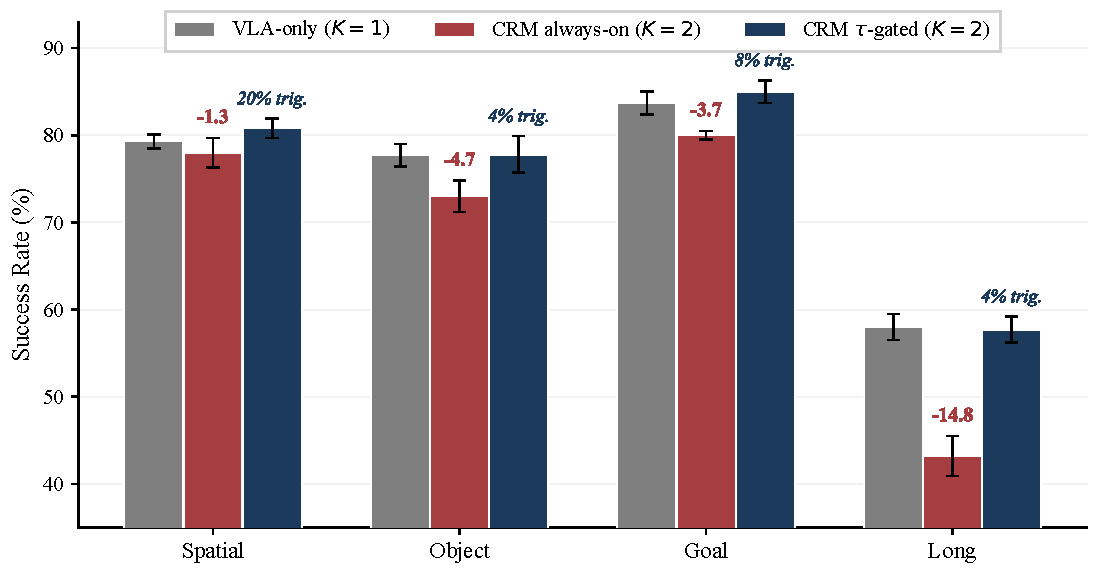
\includegraphics[width=0.8\linewidth]{fig_method_bar.pdf}
  \caption{Success rates across four LIBERO suites under the K-matched comparison. CRM always-on ($K{=}2$, red) degrades all four suites relative to VLA-only; CRM $\tau$-gated ($K{=}2$, dark blue) recovers nearly all degradation by selectively gating correction via calibrated uncertainty gating. Error bars: $\pm$1 std over $n{=}3$ seeds.}
  \label{fig:method_bar}
\end{figure}

Table~\ref{tab:main} and Figure~\ref{fig:method_bar} report task success rates. Unconditional correction degrades all four suites (Figure~\ref{fig:teaser}): $-$14.8\,pp on Long ($58.0{\to}43.2$\%), $-$4.7\,pp on Object, $-$3.7\,pp on Goal, $-$1.3\,pp on Spatial. The CRM applies a learned residual at every step, including the 80--97\% where the VLA is already confident; on these steps, corrections are noise. Calibrated $\tau$-gating recovers nearly all degradation, yielding $\Delta_{\tau\text{-gated}}$ (vs.\ VLA-only) of $+$1.5\,pp on Spatial (trigger ${\sim}$20\%), $+$1.1\,pp on Goal (trigger ${\sim}$8\%), and baseline-preserving on Object ($+$0.1\,pp, trigger ${\sim}$4\%) and Long ($-$1.3\,pp; $n{=}5$: $-$0.3\,pp$^\dagger$, trigger ${\sim}$4\%). Long, where the CRM is out-of-distribution, provides the clearest signal: unconditional correction loses 14.8\,pp; calibrated gating at ${\sim}$4\% trigger rate recovers 13.5\,pp of that degradation ($\Delta_{\mathrm{gate}}{=}{+}13.5$ vs.\ CRM always-on). An 8-seed analysis on Spatial yields $p{=}0.017$ (Appendix~\ref{sec:8seed}). Across all eight suite${\times}$VLA configurations (four SmolVLA $+$ four $\pi_{0.5}$), CRM always-on consistently degrades performance relative to VLA-only (one-sided sign test, $p = (1/2)^{8} {=} 0.004$), establishing that unconditional correction is harmful regardless of task difficulty or model scale. Moreover, 7 of 8 individual per-suite comparisons reach statistical significance at $\alpha{=}0.05$ (two-sample $t$-test, $n{=}3$ per condition); the sole exception is SmolVLA Spatial ($\Delta{=}{-}1.3$\,pp, $p{\approx}0.30$), where the small effect size ($d{=}1.0$) limits power at $n{=}3$. Gating matches or exceeds unconditional correction in 7 of 8 suite${\times}$VLA configurations (one-sided sign test, $p{=}0.035$); the single exception ($\pi_{0.5}$ Object, VLA-only 99.3\%) aligns with Rule~5. CRM degradation effect sizes are uniformly large (Cohen's $d{=}1.0$--$7.6$ on SmolVLA, $d{=}2.9$--$13.2$ on $\pi_{0.5}$), confirming that the harmful pattern is not a marginal effect.

\subsection{Correlation Between Trigger Rate and Net Improvement}
\label{sec:trigger_correlation}

\begin{wrapfigure}{r}{0.44\textwidth}
  \centering
  \vspace{-12pt}
  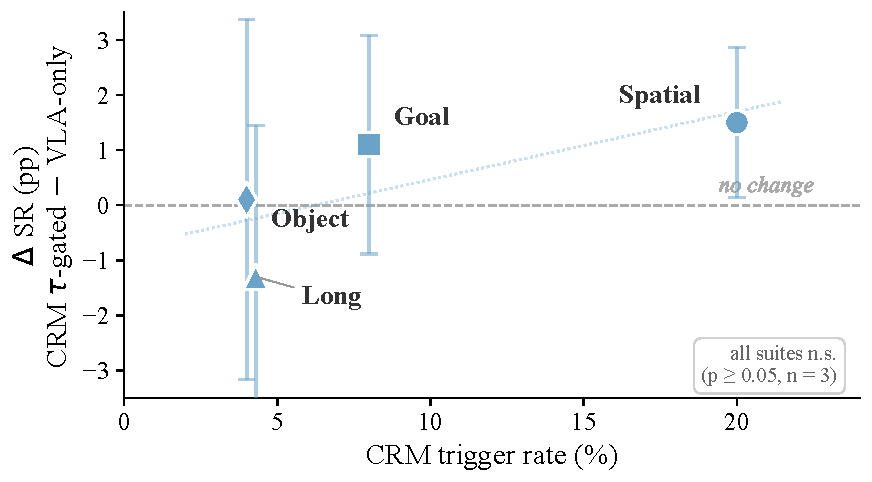
\includegraphics[width=0.42\textwidth]{fig_trigger_scatter.pdf}
  \caption{Trigger rate vs.\ improvement over VLA-only ($\Delta_{\tau\text{-gated}}$). Higher trigger $\to$ larger gain; low-trigger suites preserve baseline.}
  \label{fig:trigger_scatter}
  \vspace{-8pt}
\end{wrapfigure}

\begin{table}[t]
\centering
\caption{Cross-VLA validation on $\pi_{0.5}$ (3.6B). Unconditional CRM correction degrades all four suites, with Long suffering $-$17.5\,pp---the largest degradation across both VLAs. $n{=}3$ seeds per condition; full results including gating in Appendix Table~\ref{tab:pi05_multiseed}.}
\label{tab:pi05_main}
\small
\begin{tabular}{lccc}
\toprule
Suite & VLA-only & CRM always-on & $\Delta_{\mathrm{CRM}}$ \\
\midrule
Spatial & $98.0 \pm 0.5$ & $96.8 \pm 0.3$ & $-1.2$ \\
Object & $99.3 \pm 0.8$ & $88.0 \pm 1.0$ & $-11.3$ \\
Goal & $97.5 \pm 0.5$ & $84.5 \pm 1.3$ & $-13.0$ \\
Long & $95.0 \pm 0.9$ & $77.5 \pm 1.8$ & $\mathbf{-17.5}$ \\
\bottomrule
\end{tabular}
\end{table}

Figure~\ref{fig:trigger_scatter} visualizes the mechanism: trigger rate shows a positive trend with net improvement over VLA-only ($\Delta_{\tau\text{-gated}}$) across the four evaluated suites. Suites with high uncertainty (trigger ${>}$7\%: Spatial, Goal) see positive corrections; confident suites (trigger ${<}$5\%: Object, Long) preserve baseline, avoiding the catastrophic $-$14.8\,pp and $-$4.7\,pp degradation of unconditional correction. $\tau$-sweep analysis (Appendix Figure~\ref{fig:tau_sweep}a) shows SR varies by ${\leq}$2\,pp over a $3{\times}$ range of $\tau$, confirming that practitioners need not precisely tune the threshold. CRM corrections are robust across all magnitudes $\varepsilon \leq 0.2$ when conditioned on observation features (Appendix Figure~\ref{fig:tau_sweep}b). Notably, trigger rates are highly stable across seeds (SD ${\leq}$0.9\,pp across all suites), indicating that trigger rate is a suite-level characteristic rather than a stochastic artifact---a single validation run suffices for deployment diagnostics. This monotonic relationship makes trigger rate a zero-cost deployment diagnostic: evaluating it on a small validation set suffices to predict whether correction will yield positive gains or merely preserve baseline.

The suite-level pattern reflects task-specific uncertainty structure. Spatial tasks require precise placement relative to landmarks, producing genuinely diverse candidates when the VLA hesitates; the CRM resolves this ambiguity productively. Goal tasks involve varied goal specifications that occasionally produce uncertain predictions, yielding moderate trigger rates (${\sim}$8\%) and consistent $+$1.1\,pp gains. Object tasks involve novel instances where pretrained representations generalize well, yielding confident predictions that correction can only perturb. Long, where the CRM is out-of-distribution, confirms that gating effectiveness depends jointly on VLA uncertainty quality and CRM coverage; here the gate's conservative ${\sim}$4\% trigger rate prevents the CRM from injecting out-of-distribution noise on 96\% of steps, recovering 13.5 of the 14.8\,pp degradation.

\paragraph{Efficiency.}
Under batched inference with shared prefix encoding, $K{=}2$ latency matches $K{=}1$ (${\sim}$170\,ms), making the uncertainty probe computationally free. CRM adds ${\sim}$0.25\,ms per call; $\tau$-gating invokes it on only 4--20\% of steps (Table~\ref{tab:efficiency}).

\begin{table}[t]
\centering
\caption{Computational comparison. CRM $\tau$-gated and CRM always-on share the same $K{=}2$ VLA cost; the difference is CRM invocation frequency. CRM overhead per call is negligible (${\sim}$0.25\,ms).}
\label{tab:efficiency}
\small
\begin{tabular}{lccc}
\toprule
Method & VLA calls & Latency (ms) & CRM calls (\%) \\
\midrule
VLA-only & 1 & ${\sim}$170 & 0 \\
CRM always-on & 2 & ${\sim}$170 & 100 \\
\textbf{CRM $\tau$-gated} & \textbf{2} & $\mathbf{{\sim}170}$ & \textbf{4--20} \\
\bottomrule
\end{tabular}
\end{table}

Cross-VLA validation on $\pi_{0.5}$~\cite{black2025pi05} (3.6B) confirms with $n{=}3$ per condition that the degradation pattern persists and amplifies across model scale (Table~\ref{tab:pi05_main}): unconditional CRM correction degrades all four suites, with $-$17.5\,pp on Long---the largest degradation across both VLAs. Full results including gating are in Appendix Table~\ref{tab:pi05_multiseed}. The degradation is larger on $\pi_{0.5}$ than SmolVLA on three of four suites, suggesting that stronger base models produce more confident actions that are even more sensitive to noise injection from unconditional correction. A boundary analysis on OpenVLA-OFT~\cite{kim2024openvla} (7B, deterministic) shows that stochastic diversity is a prerequisite for multi-sample calibrated scoring: deterministic VLAs produce near-identical samples across forward passes, yielding $d_2 \approx 0$ and rendering the pairwise distance probe uninformative (Appendix~\ref{sec:applicability}). This establishes an explicit applicability boundary: the pipeline requires flow-matching or diffusion-based VLAs that produce genuinely diverse samples.

\paragraph{Deployment Guidelines.}
\looseness=-1 Our cross-suite and cross-VLA analysis yields five actionable rules:
\textit{(1)~Require stochastic VLAs.} Deterministic models produce near-identical $K{=}2$ samples, yielding $d_2 \approx 0$ (Appendix~\ref{sec:applicability}).
\textit{(2)~Train the CRM on deployment tasks.} Leave-task-out SR drops from ${\sim}$78\% to ${\sim}$2\% (Appendix~\ref{sec:reproducibility}); the CRM must cover the target task distribution.
\textit{(3)~Use trigger rate as a diagnostic.} Trigger rate ${>}$7\% predicts positive correction (Spatial $+$1.5\,pp at ${\sim}$20\%; Table~\ref{tab:main}); below ${<}$5\%, correction adds little (Object $+$0.1\,pp at ${\sim}$4\%).
\textit{(4)~$\tau$ selection is forgiving.} SR varies by ${\leq}$2\,pp over a $3{\times}$ range of $\tau$ (Table~\ref{tab:tau_sweep}); choosing a suboptimal threshold has low cost.
\textit{(5)~Do not correct near-expert VLAs.} When baseline SR exceeds ${\sim}$95\%, both unconditional and gated correction degrade performance ($\pi_{0.5}$; Tables~\ref{tab:pi05_main},~\ref{tab:pi05_multiseed}).

